\chapter{Lastimpedantie-analyse}
\label{loadanalysis}
Om een cel uit te lezen wordt er een spanning gevormd op de bitline door middel van een spanningsdeling, zoals besproken in sectie \ref{dataread}. De ene impedantie is de celimpedantie, hier valt niet veel aan te veranderen. De andere impedantie is de lastimpedantie, deze moet wel onderzocht worden zodat optimale snelheid, bitline spanningsverschil en spanningsval over de memristor resulteren.
Ook belangrijk is dat de resulterende doelstellingen robuust zijn tegen variabiliteit.

\section{Algemene lasteigenschappen en -specificaties}\label{sec:simplemodel}
In deze eerste sectie bestuderen we de spanningsdeling tussen last- en celimpedantie als een simpel model: beiden worden gemodeleerd als een eenvoudige weerstand zoals op figuur \ref{fig:dataread} in sectie \ref{dataread}. Dit model zal inzicht geven over de invloed van de weerstandswaardes op de spanningsdeling voor geheugenspecificaties zoals verschil tussen opgewekte spanning bij HRS- en LRS-cel en settlingdelay.
Een nominaal groot verschil in BL-spanning tussen een HRS- en LRS-cel is gelijk aan een relatief groot verschil tussen data- en referentiesignaal. Deze stelling gaat enkel op wanneer de referentiespanning het gemiddelde is van HRS- en LRS-dataspanning, maar dit kan zodanig gevormd worden, zoals aangehaald in sectie \ref{refread}. Een groot verschil in data- en referentiespanning is robuuster tegen de offsetspanning van de sense amplifier wanneer variabiliteit in rekening wordt genomen. In het simpele model kan het verschil in bitlijnspanning analytisch berekend worden:
\begin{equation}
 \Delta V = (\frac{R_{HRS}}{R_{last}+R_{HRS}} - \frac{R_{LRS}}{R_{last}+R_{LRS}})VDD
\end{equation} 
Voor constante waarden van $R_{HRS}$ en $R_{LRS}$ is er een maximum voor $ \Delta V$ zoals duidelijk gezien kan worden op figuur \ref{fig:rpiek}. De sensitiviteit van de last weerstand op het spanningsverschil moet men voorzichtig interpreteren. Op figuur \ref{fig:rpiek} kan gezien worden dat de helling voor het maximum stijler is dan voorbij het maximum. Het is dus beter om een iets grotere lastweerstand te hebben dan een iets te kleine lastweerstand. Wanneer men deze weerstand naar transistorafmetingen vertaalt, kan met dit op verschillend manieren realiseren. De aanweerstand van een transistor is omgekeerd evenredig met $\frac{W}{L}$. Een transistor met grote L heeft ook een grotere weerstand dan een transistor met kleine L, maar dezelfde $\frac{W}{L}$-verhouding. Voor een transistor met minimale lengte kan de grootste aanweerstand dus enkel gerealiseerd worden voor minimale breedte. Dit is gevoeliger voor variaties dan transistoren met grotere breedtes.\\
De snelheid van het opladen van de bitlijn kan in het simpele model ook analytisch beschreven worden. De volgende vergelijking stelt het tijdstip voor na het aanschakelen van de voeding wanneer de bitlijn $99\%$ is opgeladen.

\begin{align}
t = -ln(0.01)*RC \text{ met } R = (\frac{1}{R_{cel}} + \frac{1}{R_{last}})^{-1}
\end{align}

Deze delay zal kleiner worden naarmate R kleiner wordt, waarvoor een kleine lastimpedantie nodig is.

\begin{figure}[!ht]
\centering
 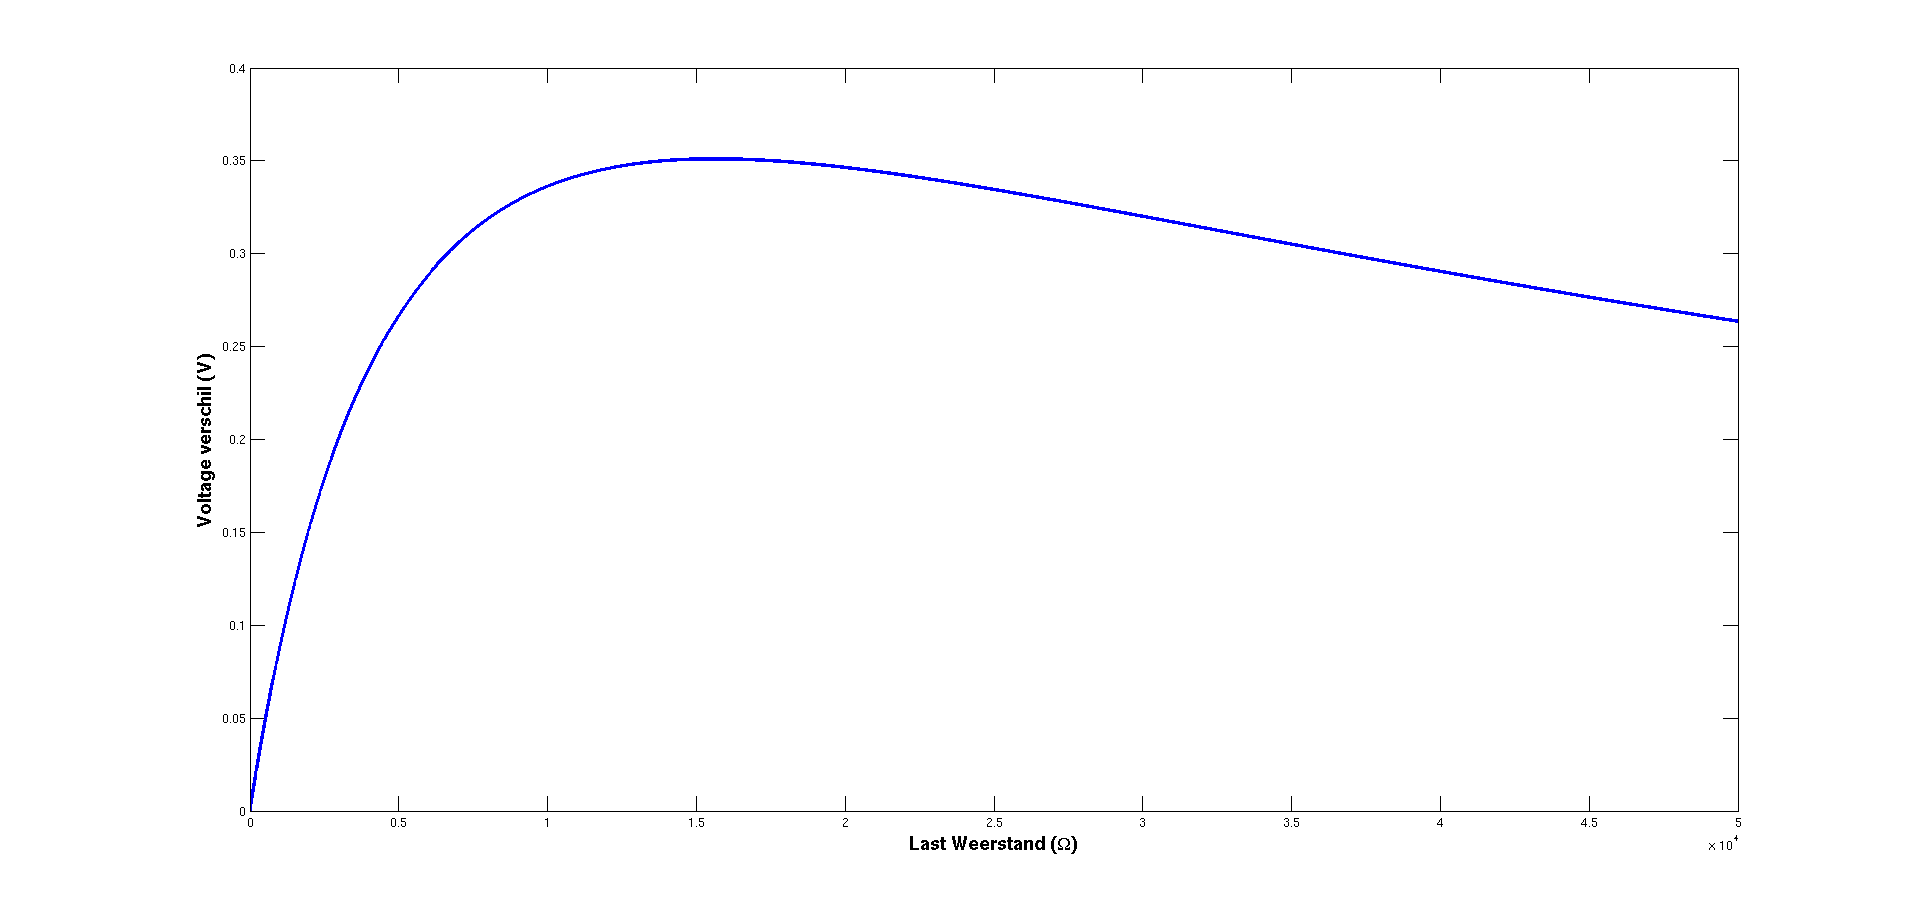
\includegraphics[width=0.80\textwidth] {../fig/hfdst-last-rpiek.png} \label{fig:rpiek}
\caption[Verschil in bitlijnspanning in functie van lastweerstand]{Verschil in bitlijnspanning in functie van lastweerstand, $R_{LRS}=7,5 k \Omega$ en $R_{HRS}= 32,5 k \Omega$}
\end{figure}




\section{Evalueren van de last}
Om verschillende lasten met elkaar te kunnen vergelijken, is het belangrijk om hun eigenschappen allemaal op dezelfde manier te bekomen. Figuur \ref{fig:simsetup} geeft de verschillende aspecten van de gebruikte simulatiesetup weer. Het testcircuit (figuur \ref{fig:simcircuit}) stelt een bitlijn voor met een capaciteit van 18fF, wat ruwweg overeenkomt met een bitlijn waaraan 100 cellen hangen. Aan deze bitlijn zijn naast de cel ook een last en een ontladinstransistor aangesloten. De ontladingstransistor is minimaal gehouden. De nominale waardes voor LRS en HRS zijn 7.5k$\Omega$ en 32.5k$\Omega$. Tijdens Monte Carlo simulaties worden deze nominale waardes als verwachtingswaarde genomen van een gaussische distributie met $\sigma = 0.833k\Omega$. Aan deze memristorweerstand hangt een WL-transistor, die ook minimaal gehouden wordt. De combinatie van deze wordt de geheugencel genoemd. De cel hangt aan de BL, WL en SL. Aan de SL is tenslotte nog een ontladingstransistor verbonden. Deze transistor wordt bewust groot gekozen zodat de equivalente weerstand van de onderste tak gedomineerd wordt door de weerstand van de geheugencel. De SL bevat ook een capaciteit van 18fF, al heeft dit geen significante invloed voor de leesbewerking, de ontladingstransistor aan de SL staat immers altijd aan. Tenslotte wordt de voedingsspanning altijd op 1V gehouden.\\\\
Figuur \ref{fig:simcontr} stelt de sequentie voor van alle controlesignalen tijdens de simulatie. Eerst wordt de bitlijn volledig ontladen. Vervolgens is er een interval waarin niets gebeurt en tenslotte wordt de last aangesloten en de bitlijn opgeladen. Op het einde van de simulatie kan men bij benadering stellen dat de BL volledig is opgeladen.\\

\begin{figure}[!ht]
\centering
\subfloat[Test circuit]{ 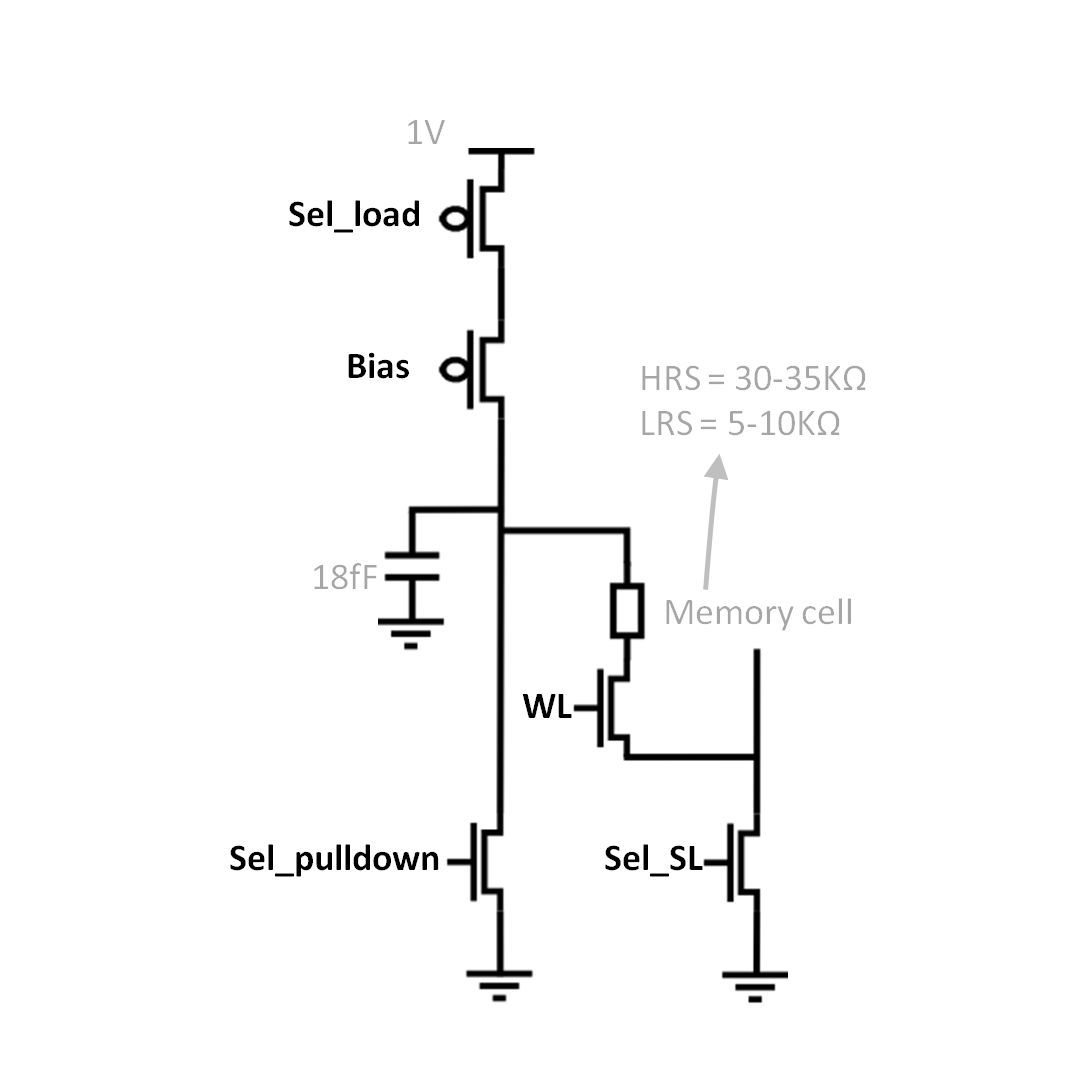
\includegraphics[width=0.45\textwidth] {../fig/hfdst-last-simsetup.png} \label{fig:simcircuit}}
\subfloat[Controle signalen]{ 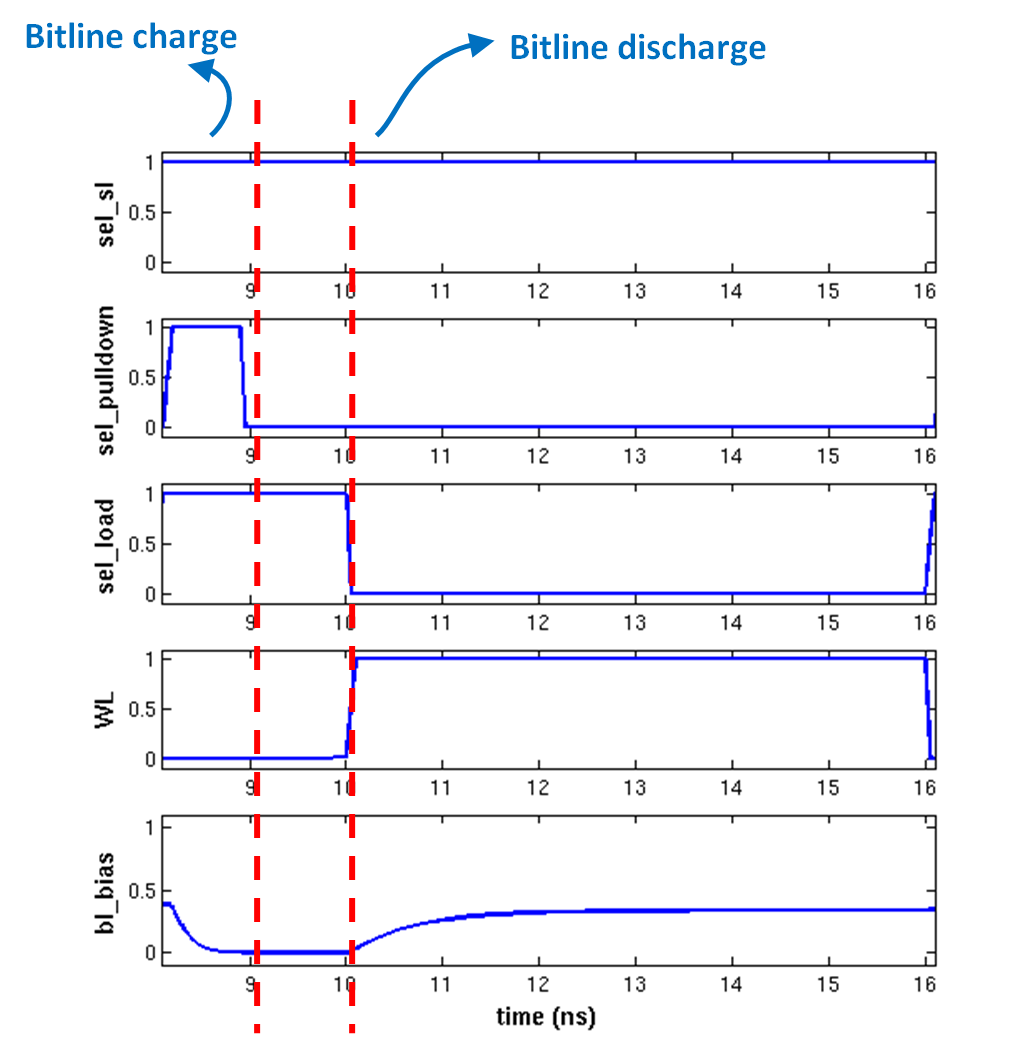
\includegraphics[width=0.45\textwidth] {../fig/hfdst-last-controlsig.png} \label{fig:simcontr}}\\
\caption[Testbench voor de lastimpedantie]{Testbench voor de lastimpedantie}\label{fig:simsetup}
\end{figure}

Eens een simulatie met een bepaalde impedantie uitgevoerd is, wordt deze last beoordeeld op vlak van resulterende oppervlakte, BL-laadsnelheid, nominaal BL-spanningsverschil en spanningsval over het geheugenelement. De oppervlakte wordt berekend op basis van de lengtes en breedtes van de lasttransistoren. De BL-laadsnelheid is de tijd die nodig is om de bitlijn $99\%$ op te laden. Het nominale BL-spanninsverschil is het verschil van de spanning over 2 BLs - aan de ene hangt een cel in HRS, de andere een cel in LRS - wanneer de bitlijn $100\%$ opgeladen is. De bitlijn wordt verondersteld $100\%$ opgeladen te zijn op het einde van de simulatie, de simulatietijd wordt voldoende hoog gehouden om dit te garanderen. De spanningsval over het geheugenelement is belangrijk wat betreft destructieve leesoperaties. Een te grote spanning gedurende een te lange tijd kan een schakeling van resistieve toestand veroorzaken. De numerieke waarde van de maximale spanningsval over de cel is heel erg afhankelijk van het type memristor. In dit onderzoek wordt uitgegaan van een maximum van 0,5V over de cel tijdens de leesbewerking\cite{ppt:model}.

\section{Vergelijking van verschillende types last}
Voor dit onderzoek worden vier mogelijke kandidaten van lastimpedanties vergeleken: de switchload (figuur \ref{fig:switchload}), de biasload (figuur \ref{fig:biasload}), de diodeload (figuur \ref{fig:diodeload}) en de bulkload (figuur \ref{fig:bulkload})\cite{bulkload}. Eerst wordt er een lineare sweep gedaan van de verschillende lasten (sectie \ref{sec:linload}), waarbij enkel de breedtes en bias spanningen worden gesweept. De lengtes van de transistoren worden minimaal gehouden om er voor te zorgen dat de transistoren binnen de pitch van de bitlijn passen. Eens variabiliteit wordt toegevoegd aan de simulatie met Monte Carlo simulaties (sectie \ref{sec:varload}) zal echter blijken dat het verschil in BL-spanning te klein is en zal de lengte van de lasttransistoren ook moeten worden vergroot (sectie \ref{sec:finaleload}).

\begin{figure}[!ht]
  \centering
  \subfloat[De switch load]{\makebox[.22\textwidth]{ 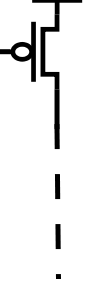
\includegraphics[width=0.12\textwidth] {../fig/hfdst-last-loadtypesswitch.png} \label{fig:switchload}}}
  \subfloat[De bias load]{\makebox[.22\textwidth]{ 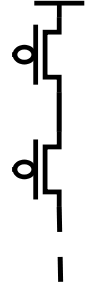
\includegraphics[width=0.12\textwidth] {../fig/hfdst-last-loadtypesbias.png} \label{fig:biasload}}}
  \subfloat[De diode load]{\makebox[.22\textwidth]{ 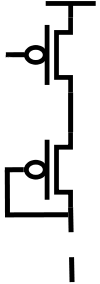
\includegraphics[width=0.12\textwidth] {../fig/hfdst-last-loadtypesdiode.png} \label{fig:diodeload}}}
  \subfloat[De bulk load]{\makebox[.22\textwidth]{ 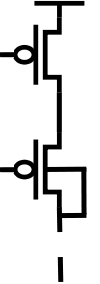
\includegraphics[width=0.12\textwidth] {../fig/hfdst-last-loadtypesbulk.png} \label{fig:bulkload}}}
  \caption[Types lastimpedanties]{De verschillende types lastimpedanties}
  \label{fig:loads}
\end{figure}

\subsection{Lineaire sweep van de lasten}\label{sec:linload}
\paragraph{}
De switchload bestaat uit \'{e}\'{e}n pMOS-transistor die volledig wordt aan- of afgeschakeld. Een lineare sweep met een transistorbreedte tussen 100nm en 500nm werd uitgevoerd en is geïllustreerd in figuur \ref{fig:switchloadsim}. Bij het vergroten van de transistorbreedte zal de aanweerstand dalen en het verschil tussen de BL-spanningen ook. Als we deze last vergelijken met het simpele model uit sectie \ref{sec:simplemodel}, zit de weerstandswaarde aan de linker kant van de piek uit figuur \ref{fig:rpiek}. Bij het vergroten van de transistorbreedte zal de BL-spanning stijgen en de spanningsval over het geheugenelement dus ook. Verder volgt de settling-tijd ook het simpele model uit sectie \ref{sec:simplemodel}, waarbij de settling-tijd daalt bij kleinere weerstandswaardes.

\paragraph{}
De biasload is een last met twee pMOS-transistoren in serie. De bovenste transistor wordt als een schakelaar gebruikt en dus volledig aan- of afgesloten. De gate van de onderste transistor wordt gebiased op een bepaalde spanning. Het voordeel van de biasload is dat men grotere weerstanden kan realiseren en dus de piek kan bereiken uit figuur \ref{fig:rpiek}. Dit kan men duidelijk zien op de x-assen van figuur \ref{fig:biasloadsim}. Ook hier zijn de breedtes van de transistoren gesweept tussen 100nm en 500nm. De biasspanning is tussen 0V en 0.4V gesweept. Een hogere biasspanning heeft geen nuttige bijdrage. Omdat de kleinste weerstand die deze configuratie kan aannemen binnen deze sweeprange net iets groter is dan die van de switchload, is de biasload ook iets trager. De oplossingen waarbij dit het geval is, hebben echter een onbruikbaar verschil in BL-spanningen. De spanningsval over het geheugenelement is vergeleken met de switchload heel wat hoger maar voor de meeste oplossingen ligt ze nog steeds onder de limiet van 0.5V.

\paragraph{}
De diodeload bestaat ook uit twee transistoren, de bovenste functioneert zoals bij de biasload als schakelaar. Bij de onderste transistor zijn drain en gate kortgesloten, dit noemt men een diode-geconnecteerde MOS-transistor. Uit de resultaten van de sweep (figuur \ref{fig:diodeloadsim}) blijkt dat de settling met deze last heel snel is, maar het BL-spanningsverschil is te klein om bruikbaar te zijn.

\paragraph{}
De bulkload werd voorgesteld in de paper van Ren et al. \cite{bulkload} als een goede kandidaat omwille van zijn grote uitgangsimpedantie. Deze last bestaat uit een schakelaartransistor en een bulk-geconnecteerde transistor. Deze bulk-geconnecteerde transistor wordt op 0V gebiased aangezien dit de beste resultaten gaf. De breedtes van de transistoren werden gevarieerd van 100nm tot 500nm. De resultaten van deze sweep zijn weergegeven in figuur \ref{fig:bulkloadsim}. In de resultaten kan gezien worden dat deze last zich vergelijkbaar gedraagt als de biasload.

\afterpage{
\begin{figure}
  \centering
  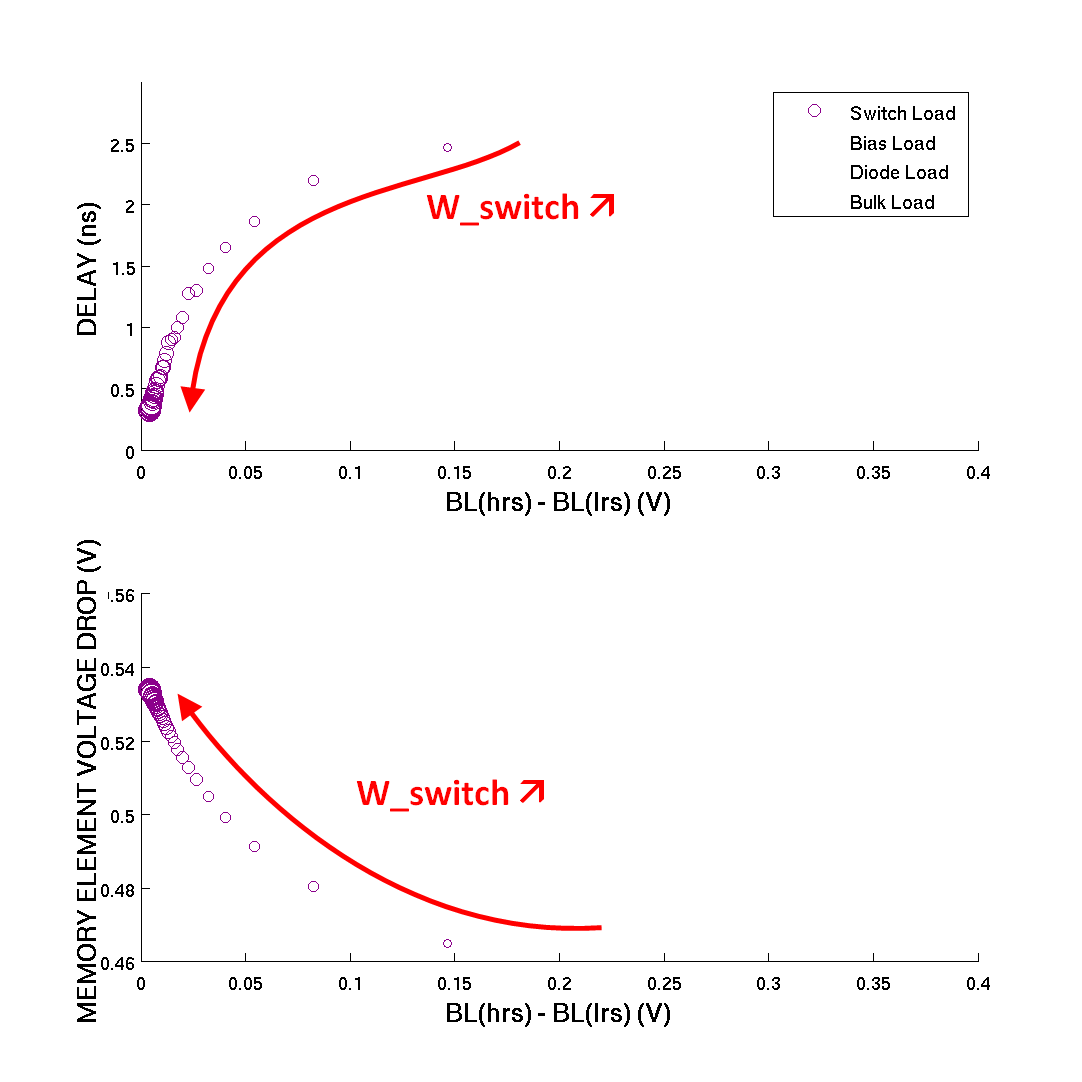
\includegraphics[width=0.67\textwidth]{../fig/hfdst-last-switchload.png}
  \caption[Lineaire sweep van switchload]{Lineaire sweep van switchload}
  \label{fig:switchloadsim}
 \centering
  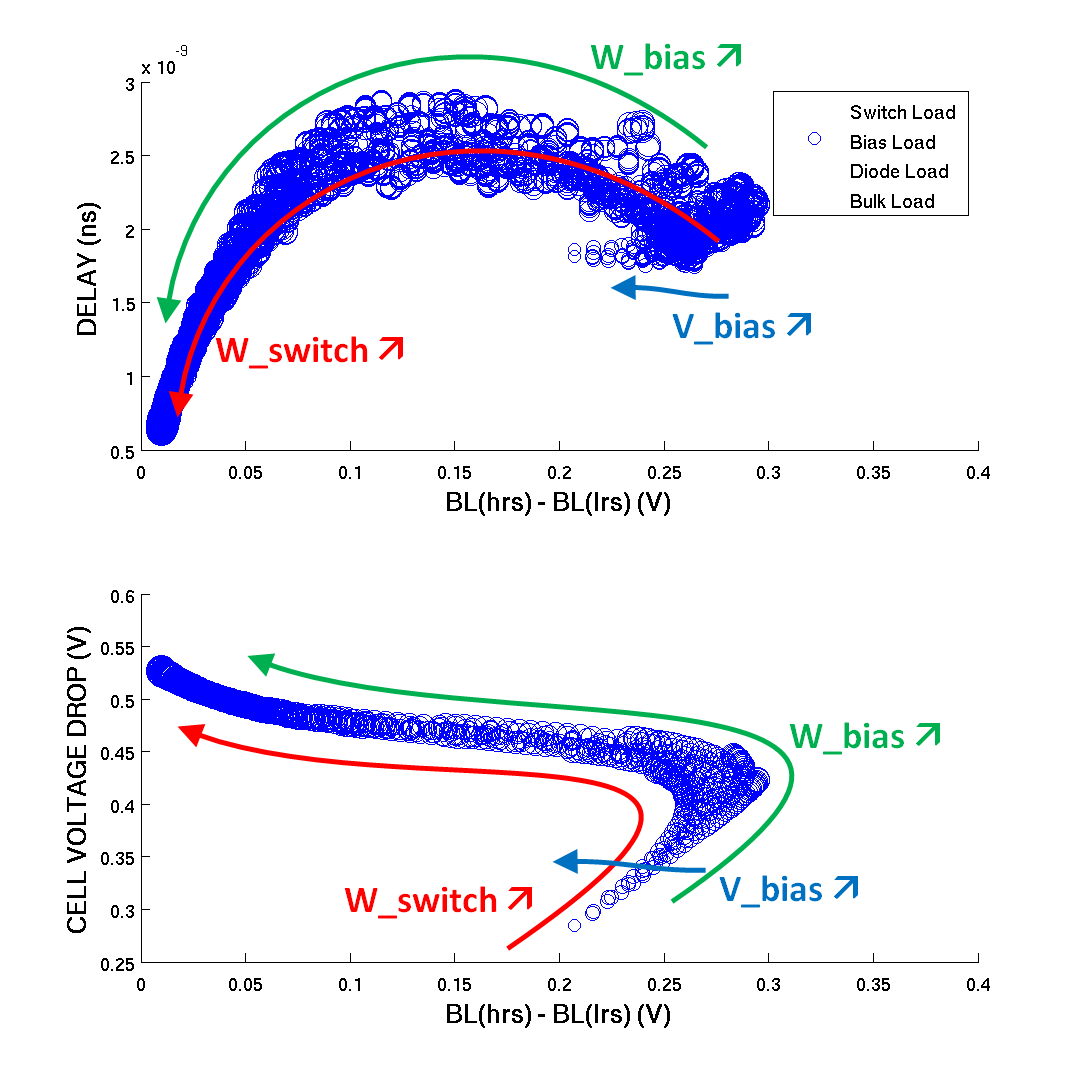
\includegraphics[width=0.67\textwidth]{../fig/hfdst-last-biasload.png}
  \caption[Lineaire sweep van biasload]{Lineaire sweep van biasload}
  \label{fig:biasloadsim}
\end{figure}
}
\afterpage{
\begin{figure}
  \centering
  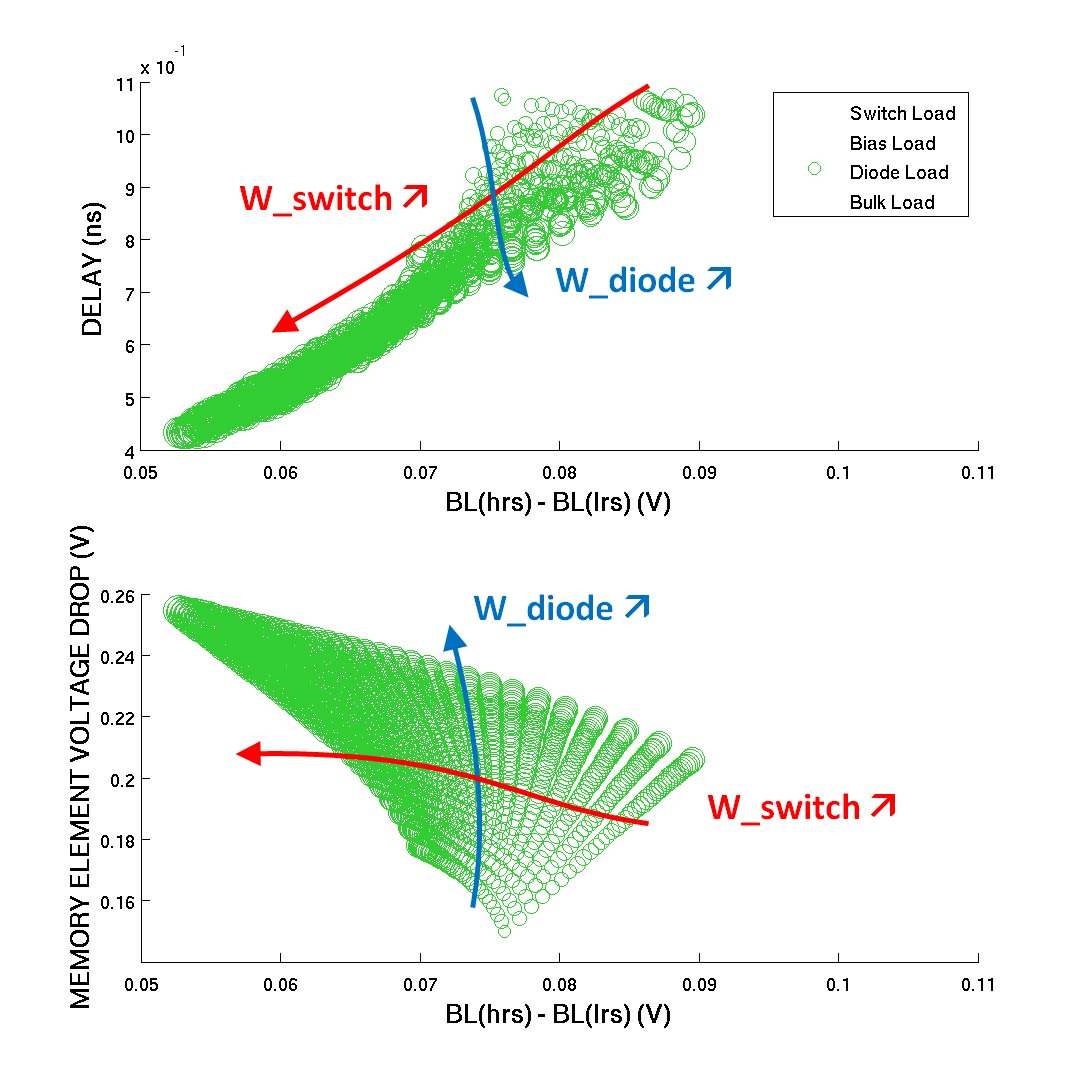
\includegraphics[width=0.67\textwidth]{../fig/hfdst-last-diodeload.png}
  \caption[Lineaire sweep van diodeload]{Lineaire sweep van diodeload}
  \label{fig:diodeloadsim}
  \centering
  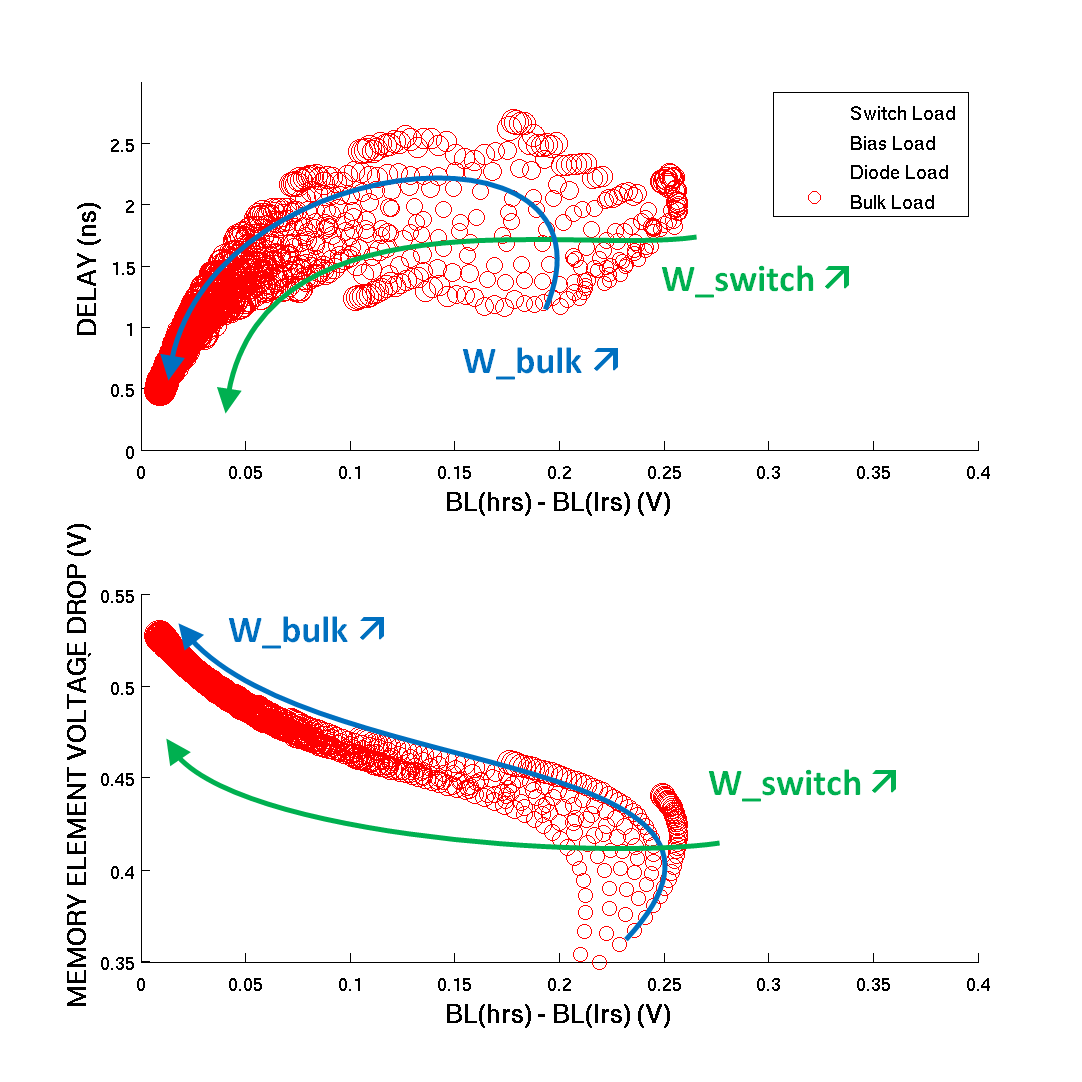
\includegraphics[width=0.67\textwidth]{../fig/hfdst-last-bulkload.png}
  \caption[Lineaire sweep van bulkload]{Lineaire sweep van bulkload}
  \label{fig:bulkloadsim}
\end{figure}
}

\subsection{Het toevoegen van variabiliteit}\label{sec:varload}
Na een selectie te hebben gemaakt van de oplossingen uit de vorige sectie, worden met deze oplossingen nieuwe simulaties gedaan waarbij ook variabiliteit in rekening gebracht wordt. De variabiliteit is toegevoegd op alle transistoren in het testcircuit en op de weerstandswaarde van de geheugenelementen. Voor de transistoren wordt er een Pelgrom constante voor Vt van $2.5mV\mu m$ gebruikt en voor $\beta$ een van $1.2\% \mu m$\cite{ppt:variatie}. Voor de weerstandswaarde van de memristors wordt er een gaussische verdeling gebruikt met verwachtingswaardes 7.5k$\Omega$ en 32.5k$\Omega$ en met $\sigma = 0.833k\Omega$. Er worden telkens 500 Monte Carlo simulaties uitgevoerd per oplossing. Hierna worden de BL-spanningen van cellen met een HRS en LRS gefit op een gaussische distributie. De oplossing met het grootste BL-spanningsverschil tussen de extrema van HRS en LRS is een biasload met een schakelaartransistorbreedte van 100nm, een biastransistorbreedte van 180nm en een biasspanning van 0V. De BL-spanning-distributies zijn geïllustreerd op figuur \ref{fig:distbias}. Uit de CDF van deze verdelingen kan men besluiten dat het BL-spanningsverschil in $99.9^2\%$ van de gevallen\footnote{$CDF(V_{BL-RHS})<0,1\%-CDF(V_{BL-LHS})>99,9\%$} groter zal zijn dan 65mV. Dit is niet bijzonder veel aangezien de distributie van de referentiespanning hier ook tussen moet passen en er daarna nog marge moet zijn voor de offsetspanning van de sense amplifier. 

\begin{figure}[!ht]
  \centering
  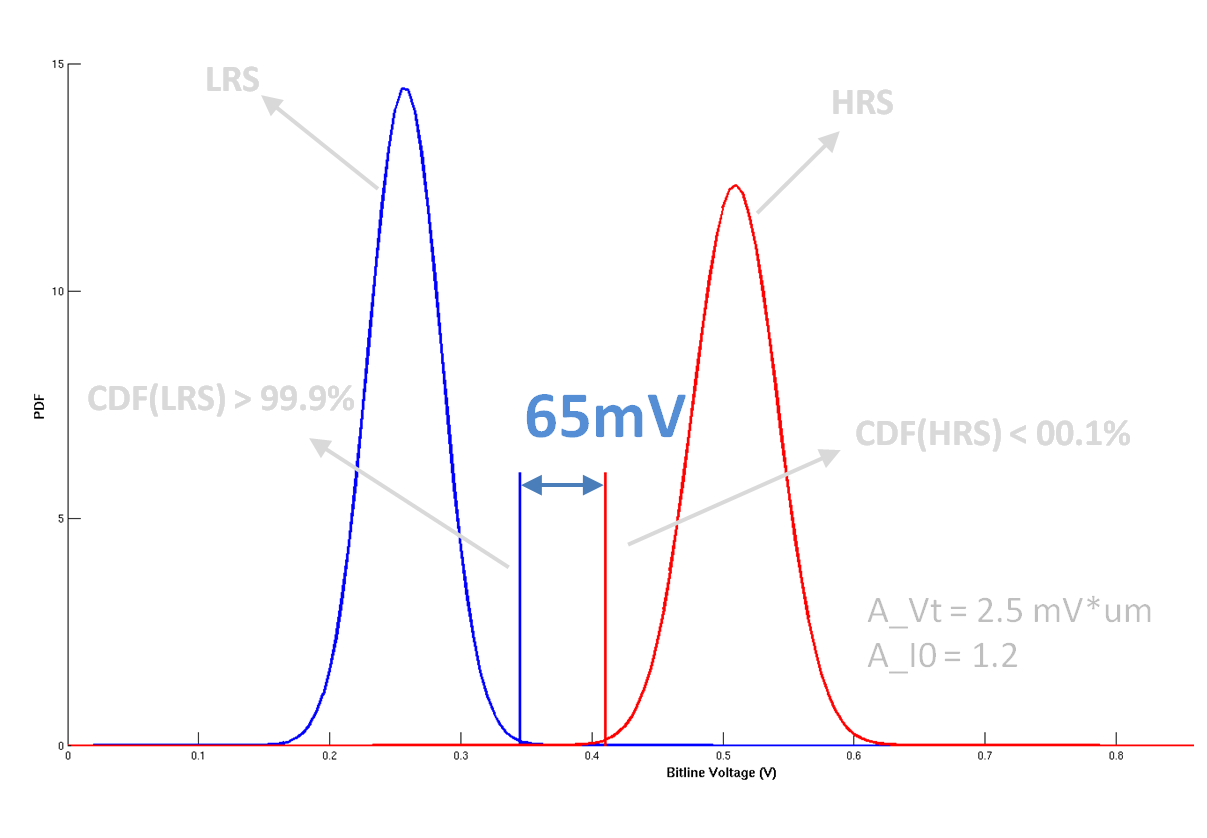
\includegraphics[width=0.67\textwidth]{../fig/hfdst-last-var1.png}
  \caption[BL-spanningsverdeling voor een biasload]{BL-spanningsverdeling voor een biasload}
  \label{fig:distbias}
\end{figure}

Figuur \ref{fig:distref} stelt de distributie van de referentiespanning voor. De verschillende curves stellen referentiesignalen opgewekt met meerdere referentiecellen [bereik 2 tot 30, steeds evenveel LRS- als HRS-cellen] voor. Zoals gezien kan worden, heeft men een groot aantal cellen nodig om een distributie breedte (6$\sigma$) van 39mV te krijgen. Dit betekent dat de offsetspanning van de SA niet groter mag zijn dan 10mV, indien de vooraf vermelde biasload gebruikt wordt. Dit is een zeer strenge voorwaarde. Daarom wordt de constraint waarbij de transistorlengte minimaal gehouden wordt, opgeheven in de volgende sectie.\footnote{Door met complementaire cellen te werken - bij elk datacel hoort een andere cel waarbij het geheugenelement zich in de andere resistieve toestand bevindt - kan het gebruik van referentiesignalen geëlimineerd worden: de SA vergelijkt in dit geval altijd een HRS-signaal met een LRS-signaal (het BL-spanningsverschil) en de offsetspanning is minder kritisch wanneer variabiliteit in rekenening wordt genomen. Voor dit soort architectuur kan dus gerust een lastimpedantie met minimale lengte worden toegepast ten koste van meer oppervlakte.}

\begin{figure}[!ht]
  \centering
  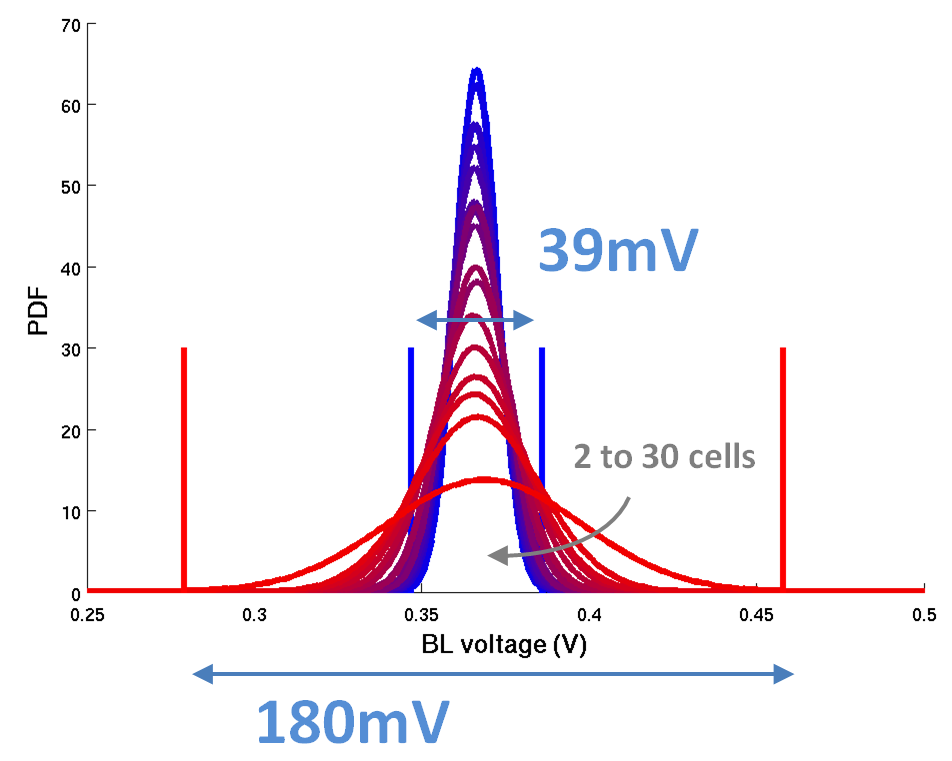
\includegraphics[width=0.67\textwidth]{../fig/hfdst-last-ref.png}
  \caption[Bitlijnspanning referentiecellen]{Bitlijn spanningsdistributies voor een verschillend aantal referentiecellen}
  \label{fig:distref}
\end{figure}


\subsection{De transistor lengte vergroten}\label{sec:finaleload}
Om de variabiliteit onder controle te houden moeten de transistoren vergroot worden. Twee opties worden hiervoor overwogen. De eerste is het toevoegen van een derde transistor in serie. Om dezelfde lastimpedantie te bekomen als voor 2 transistoren in serie, moeten de drie transistoren een grote breedte hebben. De $\frac{W}{L}$-verhouding vergroten verlaagt de aanweerstand van de individuele transistoren, maar door ze in serie te schakelen blijft de equivalente weerstand voldoende groot. Omwille van de vergrote afmetingen zouden ze bovendien minder gevoelig zijn voor mismatch. Hierbij wordt wel verondersteld dat alle drie de transistoren zich in lineair gebied bevinden. In werkelijkheid blijkt de onderste transistor zich in het near- tot subthresholdgebied te bevinden. De stroom in het subtheshold gebied varieert exponentieel met $V_{GS}-V_{T}$. De stroom en aanweerstand van de transistor zijn dus zeer gevoelig voor VT-variaties. Dit fenomeen ziet men niet bij 2 transistoren in serie, aangezien de transistoren zich hier in het lineare gebied situeren. Daarom wordt er om de mismatch onder controle te houden geopteerd voor de tweede optie, namelijk het vergroten van de transistorlengte. De lengte vergroten resulteert in een toename van de aanweerstand en vermindert variabiliteit. Omwille van de eenvoud, wordt er met deze nieuwe ontwerpkeuze teruggegrepen naar de switchload.\\
Figuur \ref{fig:length} geeft de resultaten weer van een sweep van verschillende lengtes en breedtes voor een switchload. De resultaten worden voorgesteld in functie van $\frac{W}{L}$ wat een indicatie is voor de weerstand van de transistor. In de bovenste figuur kan men duidelijk een maximum zien voor het verschil in BL-spanning zoals in sectie \ref{sec:simplemodel} werd voorspeld. Verder dient worden opgemerkt dat er een oplossing aan de linkerkant van het maximum gekozen moet worden aangezien de spanningsval over het geheugenelement van de oplossingen aan de rechterkant van het maximum te hoog zijn.
\begin{figure}[!ht]
  \centering
  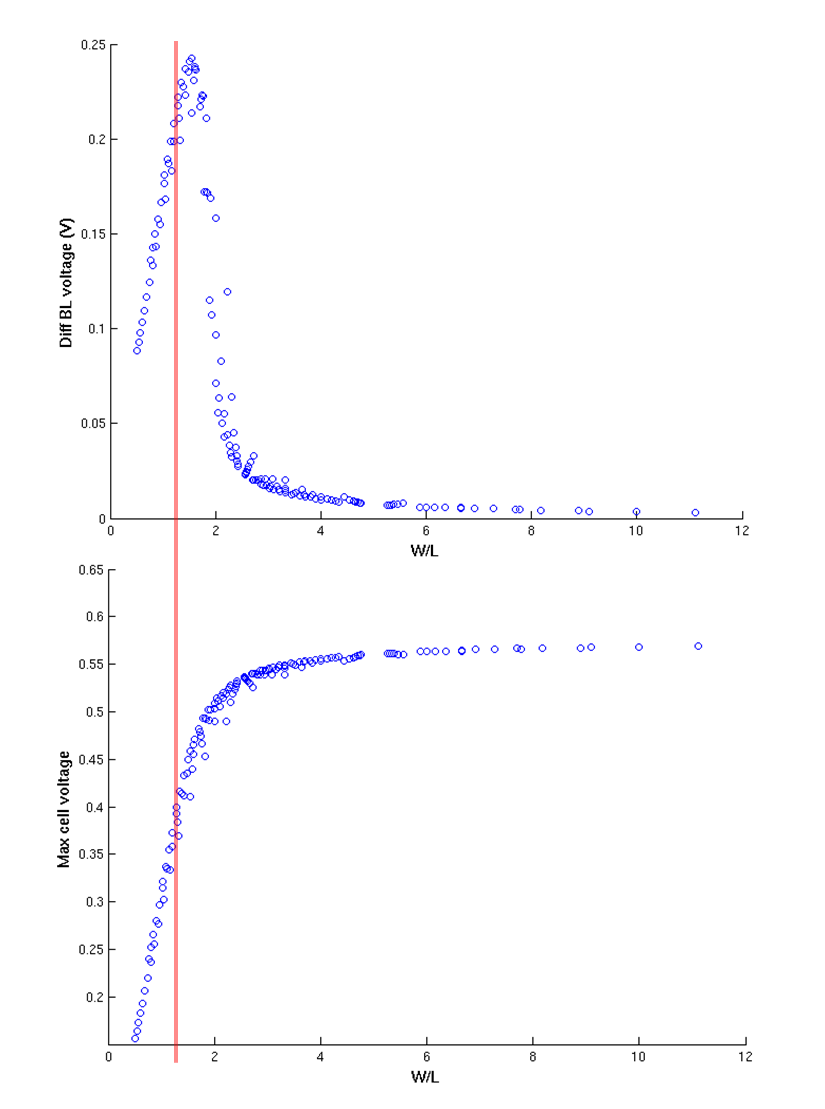
\includegraphics[width=0.65\textwidth]{../fig/hfdst-last-length.png}
  \caption[Sweep switchload over transistor lengte en breedte]{Verschillende oplossingen voor de switchload met variabele lengtes en breedtes}
  \label{fig:length}
\end{figure}

\begin{figure}[!ht]
  \centering
  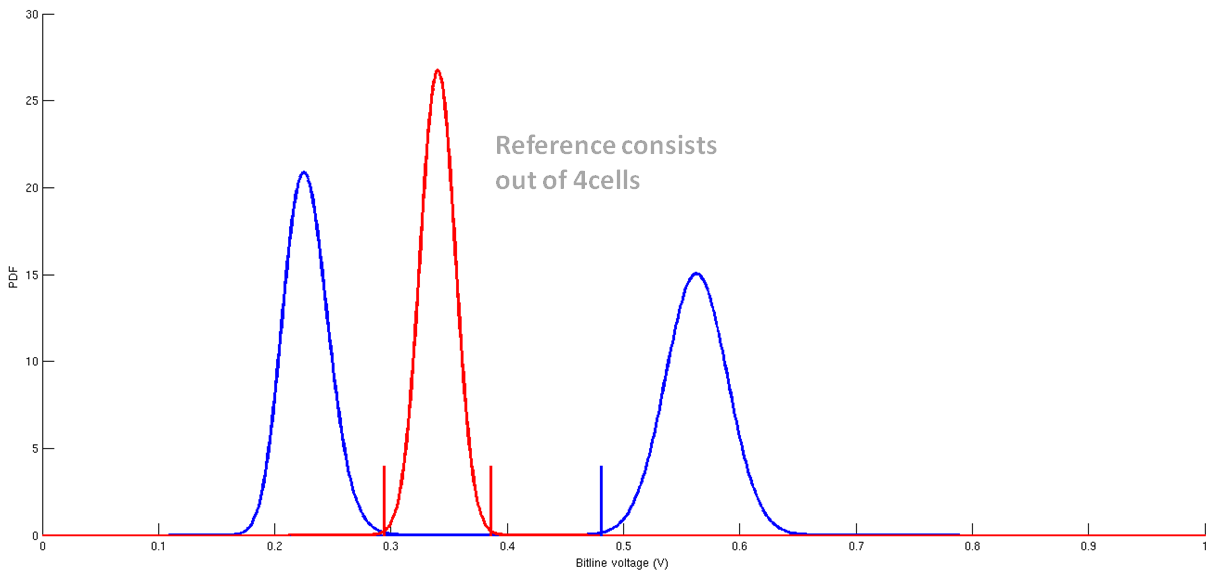
\includegraphics[width=0.65\textwidth]{../fig/hfdst-last-var2.png}
  \caption[BL-spanningsverdeling voor de finale lastimpedantie]{BL-spanningsverdeling voor de finale lastimpedantie}
  \label{fig:distswitch}
\end{figure}

Voor de finale last wordt er gekozen voor een transistor met lengte 198nm en breedte 300nm. Op figuur \ref{fig:length} wordt deze aangeduid met de rode lijn. Op figuur \ref{fig:distswitch} wordt de BL-spanningsdistributie van deze last getoond. Het minimale verschil in BL-spanning is bijna 200mV. De distributie van het referentiesignaal is ook aangegeven op deze figuur. De referentie bestaat uit 16 referentie cellen waarvan 6 in HRS en 10 in LRS. Het aantal cellen in RHS en LRS is zo gekozen dat de referentie distributie in het midden ligt tussen de distributies van de data signalen. Aangezien de standaarddeviatie op de BL-spanningen heel wat beter is, kan er gerust gekozen worden voor een last met een kleiner nominaal BL-spanningsverschil \label{anderelast}. Dit kan 2 voordelen met zich mee brengen. Zo is de spanningsval van de memristor lager wanneer men een last kiest links van het maximum in figuur \ref{fig:length}. Voor dergelijke lastimpedanties moeten de BLs bovendien tot een lagere spanning opladen wat een energie winst oplevert. Ondanks deze voordelen werd er toch geopteerd voor de oplossing met het grootste BL-spanningsverschil.

\section{Besluit}
Verschillende kandidaten voor lastimpedanties werden overwogen. Aanvankelijk werd er getracht een last met minimale transistorlengtes te vinden, dit bleek echter niet haalbaar wanneer variabiliteit in rekening wordt genomen. Een enkele transitor met niet-minimale afmetingen bleek de beste resultaten te leveren wat betreft BL-spanningsverschil en spanningsval over geheugenelement. Deze voorwaarden stroken echter met settling tijd minimaliseren. Het BL-spanningsverschil en de spanningsval van het gehegeugenelement zijn wel prioritair, dus werd er niet geoptimaliseerd voor delay.
